% %%%%%%%%%%%%%%%%%%%%%%%%%%%%%%%%%%%%%%%%%%%%%%%%%%%%%%%%%
% | - Structural analysis of IrO2 and IrO3 oxides %%%%%%%%%
% %%%%%%%%%%%%%%%%%%%%%%%%%%%%%%%%%%%%%%%%%%%%%%%%%%%%%%%%%
% TODO: Synthax for calling subplots in figure Figure 1.d or Figure 1.d)
% TODO: "we note that ..." is used a few times Kirsten
%
% Important Points:
%   * A good candidate set is a set of materials that have a large degree of 'structural diversity'
%
%   * We can make an analogy between the shape of these plots and typical van-der Waals curves
%     * I would argue that the tails are much less steep than a van-der Waals curve because in most cases the there is still a large degree of bonding
%       * Essentially these systems can create more and more 'porous' structures as the density is decreases, which allows us to get really large porous structures
%         * A good point can be made here that these types of systems could be useful for battery applications
%           * Pores are good in this context I think?
%
%
%   * The main coordination environments are 6 and 4-fold coordinated (Ir-O4/6 units)
%     * This is consistent with crystal field theory, or literature, etc.
%     * 6/4-coord accounts for TEMP percent of the IrO2/3 candidate space
%       * TODO Get these numbers
%     * There are in addition to 6/4-coord, a lot of other types of coordination environments
%       * A lot of these are simply weird, aphysical structures for sure
%         * Unassociated oxygens
%           * Singly-associated (part of N-hedra)
%           * Completely un-unassociated O atoms, just randomly placed in unit cell
%
%         * Especially at the extreme ends of the average coord metric
%       * But there are also a lot of legitimate coordination environments
%         * I've manually parsed the dataset and found
%
%   * There is a lot to say about the different kinds of 100% corner sharing octahedral IrO3 systems
%     * There are a lot of these systems that differ in subtle ways
%       * Basically octahedra can be "rotated" in different directions, making them distinct
%
%   * Interesting types of systems
%     * Layered systems (A lot of variety here)
%     * Cubic coordination environments (A few cool looking examples)
%     * New coordination environments
%       * TODO Remind myself again of these
%
%   * IrO2 has more 4-fold coordinated systems than IrO3
%     * Makes sense, the more oxygens you have the more oxygen-rich motifs are favored
%   * IrO2 has large "dip" in the EvsV "convex hull" while IrO3 has a much more shallow increase in energy as you move to the right from the most stable polymorph
%     * This is probably due to the fact that IrO3 can create more porous layered structures
%
% NOTES:
%   * Describe convex hull, classes of structures (\ce{$\alpha$-AlF3} like, rutile like, and layered, should be segregated in hull plot)
%   * Describe structures within each class, cite lit where appropriate
% __| %%%%%%%%%%%%%%%%%%%%%%%%%%%%%%%%%%%%%%%%%%%%%%%%%%%%%



% %%%%%%%%%%%%%%%%%%%%%%%%%%%%%%%%%%%%%%%%%%%%%%%%%%%%%%%%%
% ####################### Paragraph #######################
% %%%%%%%%%%%%%%%%%%%%%%%%%%%%%%%%%%%%%%%%%%%%%%%%%%%%%%%%%
% TEMP
%
% There should be a paragraph which discussed the structural drift and performance/acceleration in more detail
% I would use the updated version of Figure 2c.
% %%%%%%%%%%%%%%%%%%%%%%%%%%%%%%%%%%%%%%%%%%%%%%%%%%%%%%%%%
% | - %%%%%%%%%%%%%%%%%%%%%%%%%%%%%%%%%%%%%%%%%%%%%%%%%%%%%
%
As a next step we assess the stability as well as the structural variety of the DFT optimized structures, consisting of 381 \IrOtwo and 185 \IrOthree unique polymorphs.
%
% Why do we show this plot, motivate earlier/here
Figure~\ref{fig:E_vs_V} a and b shows the DFT computed enthalpy of formation for \IrOtwo and \IrOthree plotted against the inverse density.
%
To obtain a physically meaningful cutoff for the enthalpy of formation, we computed the metastability limits for \IrOtwo and \IrOthree relative to their amorphous phases using the methodology of Persson \latin{et. al.}~\cite{Aykol2018}.
%
Further computational details can be found in the Supporting Information.
%
The metastability limit for both \IrOtwo and \IrOthree were comptuted to occur at an enthalpy of formation of -0.34 eV/atom and are displayed as horizontal lines in Figure~\ref{fig:E_vs_V}a and b.
%
There are 195 and 74 polymorphs for \IrOtwo and \IrOthree, respectively, that are within the meta-stability line, and can therefore, in principle be synthesized.
%
% These last two sentences can be removed
%These values are almost identical, possibly indicating that the energy of the amorphous phases are insensitive to the exact stoichiometry.
%
%Measuring the metastability relative to the hull for each stoichiometry yields a metastability window of 0.5 and 0.3 eV/atom for \IrOtwo and \IrOthree, respectively.
% __| %%%%%%%%%%%%%%%%%%%%%%%%%%%%%%%%%%%%%%%%%%%%%%%%%%%%%


% =========================================================
% FIGURE ==================================================
% | - Figure | Energy vs. Volume (motif distribution)
\begin{figure*}[!htb]
\centering
\makebox[\textwidth][c]{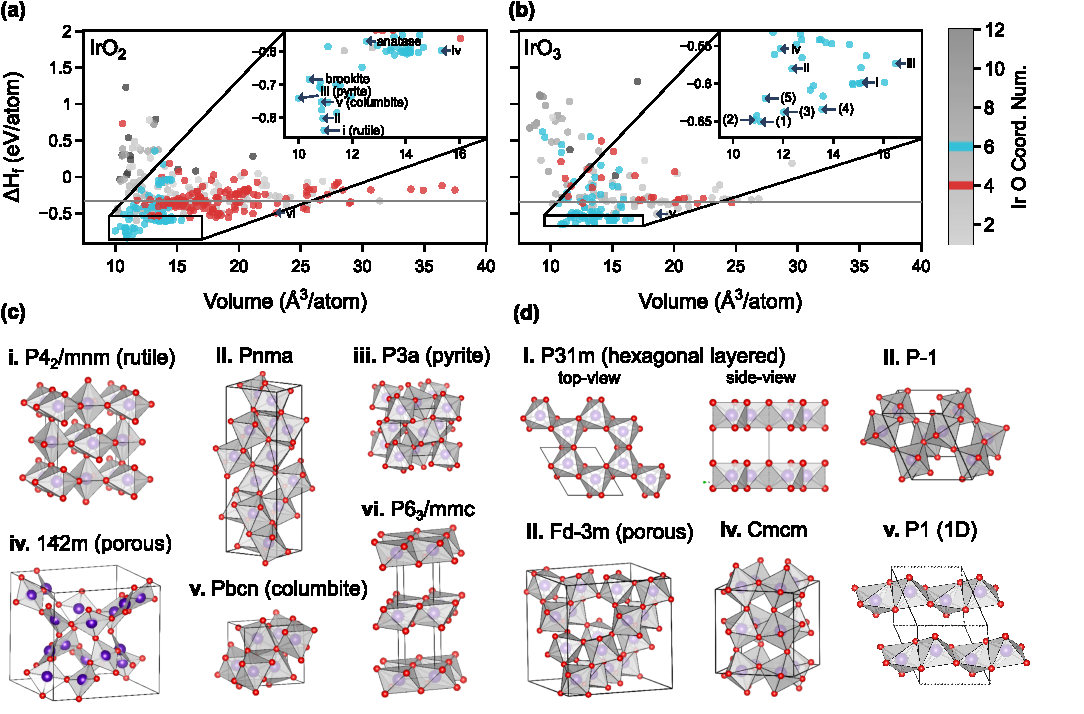
\includegraphics[
width=\textwidth,height=\textheight,keepaspectratio]
{02_figures/e_vs_v_motifs.pdf}
}
\caption{\label{fig:E_vs_V}
%381 \IrOtwo and 185
Enthalpy of formation for the \num{381} \IrOtwo (a) and \num{185} \IrOthree (b) DFT optimized structures in the candidate data set plotted against the volume per atom.
%
Insets in the low energy region for (a) and (b) are shown.
%
The color bar represents the average coordination number between Ir and O, with the most common, 6 (octahedra) and 4 (tetrahedral) coordinations, highlighted.
%
For \IrOtwo (c) and \IrOthree (d) we highlight the structures of select polymorphs.
}
\end{figure*}
% __| =====================================================
% =========================================================


% %%%%%%%%%%%%%%%%%%%%%%%%%%%%%%%%%%%%%%%%%%%%%%%%%%%%%%%%%
% ####################### Paragraph #######################
% %%%%%%%%%%%%%%%%%%%%%%%%%%%%%%%%%%%%%%%%%%%%%%%%%%%%%%%%%
% TODO Say that the \IrOthree bulk phase corresponds to the o-covered regime
% There is a large variety in density on this plot
% IrO3 has a small dependance on the volume
% %%%%%%%%%%%%%%%%%%%%%%%%%%%%%%%%%%%%%%%%%%%%%%%%%%%%%%%%%
% | - %%%%%%%%%%%%%%%%%%%%%%%%%%%%%%%%%%%%%%%%%%%%%%%%%%%%%
To increase the likelihood of discovering novel material types it is desirable that our candidate space be structurally diverse, with materials that span a large range of densities and coordination environments.
%
We note that for both compositions, there is a large variety in density such that both low volume (dense) and high volume (porous) structures are contained in the data set.
%
The highest density structures corresponds to an atomic packing factor of roughly 0.50, and are where the most stable structures are found.
%
On the other end, the lowest density systems sampled have atomic packing factors as low as 0.15.
%where the shape of envelope curve (lowest energy for a given volume) is analogous to the shape of the Lennard-Jones potential. \textbf{is this important or expected?}
%
% NOTE Can make a comment about the fact that these porous species may be over-stabilized with PBE DFT
However, for \IrOthree there is a comparatively weaker relationship between the energy and volume,
such that even highly porous structure are within 0.1 eV of the most stable phase. 
%
% What is the error in estimated energy?
The stability of highly porous systems have a tendency to be overestimated on the DFT+GGA level, due to missing van der Walls interactions \cite{}. 
%
% COMBAK Explain this point better, this has to do with the oxidation state, coordination preservation rules that I've been playing around with
%
%This property is likely due to the fact that \IrOthree's oxidation state can more can form readily form layered or porous structures.
%
% \textbf{unclear what you mean here, vdw is attractive so shouldn't it just make them more stable?}
%
%Although formation energies for highly porous systems tend to be over stabilized at the DFT+GGA level of theory because of the improper description of van der Walls interactions, the magnitude of these errors \textbf{don't severely impact the results or something}
% __| %%%%%%%%%%%%%%%%%%%%%%%%%%%%%%%%%%%%%%%%%%%%%%%%%%%%%

% ####################### Paragraph #######################
% %%%%%%%%%%%%%%%%%%%%%%%%%%%%%%%%%%%%%%%%%%%%%%%%%%%%%%%%%
% Explaining coordination motif distribution (octahedral, tetrahedral
% %%%%%%%%%%%%%%%%%%%%%%%%%%%%%%%%%%%%%%%%%%%%%%%%%%%%%%%%%
% | - %%%%%%%%%%%%%%%%%%%%%%%%%%%%%%%%%%%%%%%%%%%%%%%%%%%%%
%
All structures have been classified with respect to the Ir-O coordination environment (such as octahedral, square pyramidal, tetrahedral, cubic, etc.),
by using the chemEnv package, developed by Waroquiers et. al. \cite{Waroquiers2017} as implemented in the Pymatgen software \cite{Ong2013}.
%
Although the dataset was found to contain a large range of coordination environments ranging from 2 to 10,
structures with a coordination number of 6 (octahedral) or 4 (tetrahedral) were found to be most prevalent
% (accounting for roughly TEMP percent of all structures)
and have been highlighted in blue and red respectively in Figure~\ref{fig:E_vs_V}a and b.
%
For both \IrOtwo and \IrOthree the vast majority of most stable (within 0.1 eV) structures adopt an octahedral coordination environment, a common coordination motif found to be favorable in many other transition metal oxides.\cite{Waroquiers2017}
%
% This has to be expanded upon or else maybe dropped, we can discuss
% I don't understand the end of this sentence.  Give some information of how this applies to your structures.
% I've added a sentence at the end where we simply describe whether our most stable structures are corner vs edge sharing
The arrangement of the octahedral units, which are connected through either corner-, edge sharing,
can furthermore be used to classify the structures, that typically has a combination of the two.
%
% Look into this deeper, there is probably a difference in fraction of mixed corner+edge between IrO2 and IrO3
Of the top 10 \IrOtwo and \IrOthree structures, 9/10 of \IrOtwo and 5/10 of \IrOthree have a mixed corner and edge sharing octahedral packing.
%
This demonstrates that \IrOtwo prefers to form edge sharing octahedra as a result of having to share more oxygens to maintain its stoichiometry.
%
\IrOthree has comparatively more oxygens per unit cell, and as such can adopt completely corner sharing arrangements similar to cubic perovkite-type structures.
% __| %%%%%%%%%%%%%%%%%%%%%%%%%%%%%%%%%%%%%%%%%%%%%%%%%%%%%

% ####################### Paragraph #######################
% %%%%%%%%%%%%%%%%%%%%%%%%%%%%%%%%%%%%%%%%%%%%%%%%%%%%%%%%%
% TEMP
% %%%%%%%%%%%%%%%%%%%%%%%%%%%%%%%%%%%%%%%%%%%%%%%%%%%%%%%%%
% | - %%%%%%%%%%%%%%%%%%%%%%%%%%%%%%%%%%%%%%%%%%%%%%%%%%%%%
Figure~\ref{fig:E_vs_V}c,d shows a selection of meta-stable structures is shown for \IrOtwo and \IrOthree respectively.
%
For \IrOtwo, we found the rutile structure to be the most stable,
in agreement with experimental and known crystalographic data.
%
Additionally, the experimentally synthesized high pressure pyrite phase of \IrOtwo was found in our dataset and has a formation enthalpy TEMP greater than rutile, in agreement with experimental calorimetric data.~\cite{bolzan1997structural, shirako2014synthesis}
%
% where only the rutile and pyrite phases are reported to have been synthesized \cite{bolzan1997structural, shirako2014synthesis}, the pyrite phase also predicted to be metastable in this work. 
%
In addition, several common \ABtwo crystal structures were found within the dataset, including columbite~\cite{columbite}, brookite~\cite{brookite} and anatase~\cite{anatase} phases
(all bulk structures can be viewed online at catalysis-hub.org).
%
For \IrOthree the five most stable systems were shown in Figure~\ref{fig:iro2_al}, and have been labeled with numbers (1)-(5) in Figure~\ref{fig:E_vs_V} b.
%
We have identified several interesting meta-stable structures, including two dimensional(i), highly porous(iii) and on dimensional(v) polymorphs with varying degrees of porosity and connectivity,
which is important for applications as battery cathodes or ionic conductors.\cite{}
% which could be interesting for battery applications .
%
% \textbf{the labeling scheme jumping between two figures is a little confusing here, and it obfuscates the point I think you are trying to make in this last sentence}
%
% COMBAK
Interestingly, the most stable \IrOthree structure in the MP dataset~\cite{mp-1097041} corresponds to the TEMP th most stable \IrOthree polymorph in our dataset
(iv in Figure~\ref{fig:E_vs_V}d with a Cmcm space group), 
meaning that we have uncovered TEMP new and more stable \IrOthree structures than previously known.
% __| %%%%%%%%%%%%%%%%%%%%%%%%%%%%%%%%%%%%%%%%%%%%%%%%%%%%%
